\documentclass{beamer}

\usepackage[ngerman,english]{babel}
\usepackage{listings}

\usepackage[utf8x]{inputenc}
\usepackage{xcolor}
\setbeamertemplate{bibliography item}{\insertbiblabel}
\usepackage{multimedia}
\usepackage{setspace}
\usepackage{appendixnumberbeamer}
\usepackage{tabularx}
\usepackage{rotating}
\usepackage{multirow}
\usepackage{extrabeamercmds}

\definecolor{lightBlue}{rgb}{0.62,0.71,0.91}
\definecolor{darkBlue}{rgb}{0.08,0.15,0.44}

\definecolor{one}{rgb}{0.28,1,0}
\definecolor{two}{rgb}{0.63,1,0}
\definecolor{three}{rgb}{1,0.99,0}
\definecolor{four}{rgb}{1,0.99,0}
\definecolor{five}{rgb}{1,0.52,0}
\definecolor{six}{rgb}{1,0,0}

% Keine Knöpfe
\beamertemplatenavigationsymbolsempty
% Basisfarbe
\def\swidth{2cm}
\usetheme[width=\swidth]{Hannover}

\setbeamercolor{frametitle}{fg=white,bg=darkBlue}
\setbeamercolor{block body}{fg=white, bg=darkBlue}
\setbeamercolor{sidebar}{bg=lightBlue}
\setbeamercolor{section in head/foot}{fg=black}
\setbeamercolor{author in head/foot}{fg=black}
\setbeamercolor{date in head/foot}{bg=lightBlue, fg=black}
\setbeamercolor{structure}{bg=darkBlue, fg=darkBlue}

\setbeamercolor{normal text}{bg=black,fg=black}
\setbeamercolor{section in sidebar}{fg=black}
%\setbeamercolor{author in sidebar}{fg=darkBlue}
\setbeamercolor{section in sidebar shaded}{fg=gray!80}
\setbeamercolor{subsection in sidebar}{fg=black}
\setbeamercolor{title in sidebar}{fg=black}
\setbeamercolor{subsection in sidebar shaded}{fg=gray}

\setbeamercolor{background canvas}{bg=white}
\setbeamercolor{block body alerted}{bg=normal text.bg!90!black}
\setbeamercolor{block body example}{bg=normal text.bg!90!black}
\setbeamercolor{block title}{bg=darkBlue, fg=white}
\setbeamercolor{block title example}{use={normal text,example text},fg=example text.fg!75!normal text.fg,bg=normal text.bg!75!black}
\setbeamercolor{title}{fg=white}
\setbeamercolor{titlelike}{fg=black}

\useinnertheme{circles}

\setbeamertemplate{footline}
{
\leavevmode%
\hbox{%
\begin{beamercolorbox}[wd=0.156\paperwidth,ht=2.25ex,dp=1ex,center]{date in head/foot}% % .333333
	\usebeamerfont{date in head/foot}
	\insertframenumber{} von \inserttotalframenumber \hspace*{2ex}%/ \hspace*{2ex}
\end{beamercolorbox}}%
\vskip0pt%
} 

\title{Summary of ''The Curious Case of the PDF
Converter that Likes Mozart: Dissecting and Mitigating the Privacy Risk of Personal Cloud Apps``} % [The Curious Case of the PDF Converter that Likes Mozart]
%\subtitle{Hamza Harkous, Rameez Rahman, Bojan Karlas and Karl Aberer}
\author{Jens Becker, Katharina Mulack, Simon Weidmann}
\institute{Security of complex Information systems}
\date{17. January 2018}

\begin{document}
{
\section*{}
\frame{\titlepage}
}

{
\section*{}
	\begin{frame}
	\frametitle{Contents}
      \tableofcontents    
\end{frame}
}

{
\section*{}
	\begin{frame}
      \begin{center}
        \font\endfont = cmss10 at 10.40mm
        \color{darkBlue}
        \endfont 
        \baselineskip 20.0mm   
        Preface 
      \end{center}    
\end{frame}
}

\section{Preface}
\frame{
	\frametitle{Preface}	
}

%{
%\section*{}
%	\begin{frame}
%      \begin{center}
%        \font\endfont = cmss10 at 10.40mm
%        \color{darkBlue}
%        \endfont 
%        \baselineskip 20.0mm   
%        Introduction
%      \end{center}    
%\end{frame}
%}

%\section{Introduction}
%\frame{
%	\frametitle{Introduction}
%	Examination of ''over-privileged`` third party apps for Google Drive \vspace{5mm} \\
%	Suggestion of new permission models \vspace{5mm} \\
%	Introduction of an app store \vspace{5mm} \\
%	Analysis of the behaviour of app developers \vspace{5mm} \\
%	Suggestion of best practices
%}
%\frame{
%	\frametitle{Introduction}
%}

{
\section*{}
	\begin{frame}
      \begin{center}
        \font\endfont = cmss10 at 10.40mm
        \color{darkBlue}
        \endfont 
        \baselineskip 20.0mm   
        New permission models 
      \end{center}    
\end{frame}
}

\section{New permission models}
\frame{
	\frametitle{New permission models}
	Delta Permissions (DP) \vspace{5mm} \\
	Assumption: Users are detained if told which permissions are unnecessary 
}
\frame{
	\frametitle{New permission models: DP}
	\begin{center}
    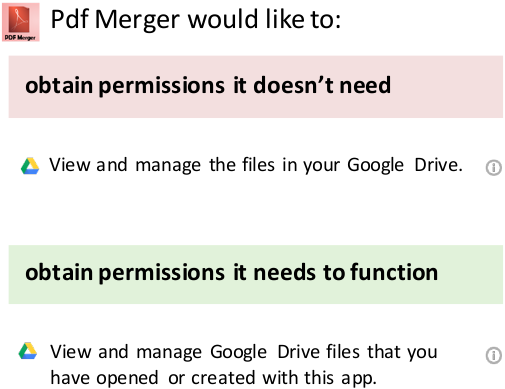
\includegraphics[width=0.7\textwidth]{images/dpExample.png}\cite{paper} % , height=0.7\textheight
    \end{center}
}
\frame{
	\frametitle{New permission models}
	Immediate Insights (IM) \vspace{5mm} \\
	Assumption: Users are detained if told which informations can be gained 
}
\frame{
	\frametitle{New permission models: IM}
	\begin{center}
    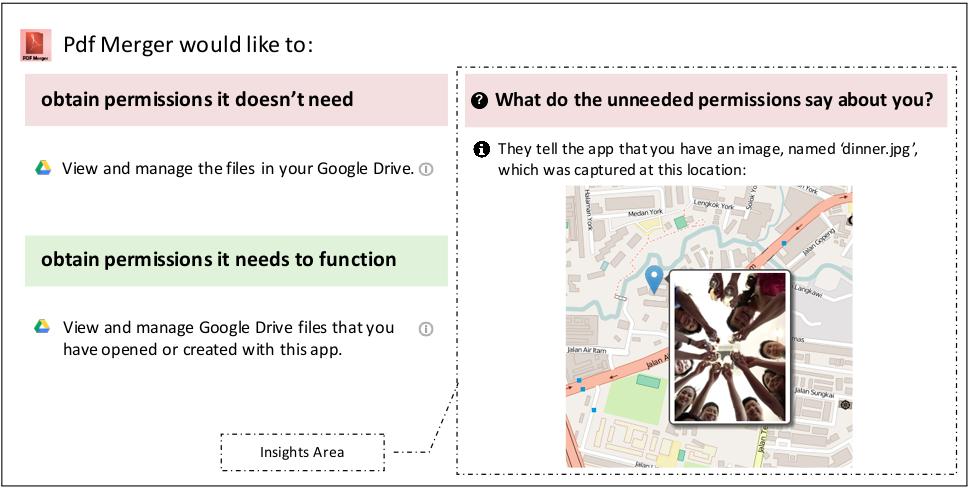
\includegraphics[width=1\textwidth]{images/imExample.png}\cite{paper} % , height=0.8\textheight
    \end{center}
}
\frame{
	\frametitle{New permission models}
	Far-reaching Insights (FR) \vspace{5mm} \\
	Assumption: Users are detained if told which far reaching insights can be gained 
}
\frame{
	\frametitle{New permission models: FR}
	\begin{center}
    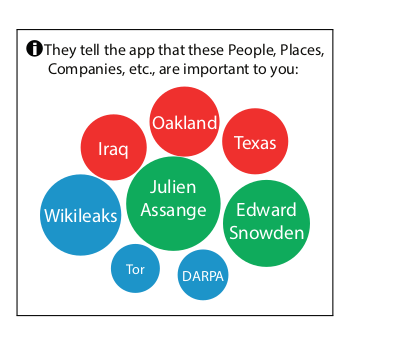
\includegraphics[width=0.8\textwidth]{images/fr1.png}\cite{paper} % , height=0.8\textheight
    \end{center}
}
\frame{
	\frametitle{New permission models: FR}
	\begin{center}
    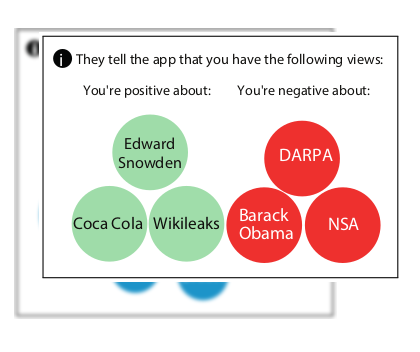
\includegraphics[width=0.8\textwidth]{images/fr2.png}\cite{paper} % , height=0.8\textheight
    \end{center}
}
\frame{
	\frametitle{New permission models: FR}
	\begin{center}
    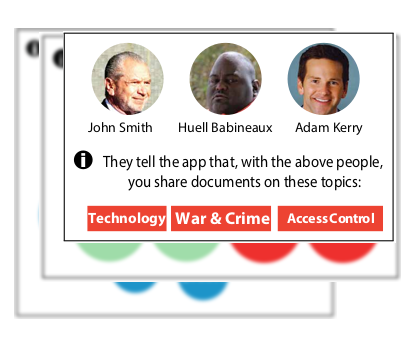
\includegraphics[width=0.8\textwidth]{images/fr3.png}\cite{paper} % , height=0.8\textheight
    \end{center}
}
\frame{
	\frametitle{New permission models: FR}
	\begin{center}
    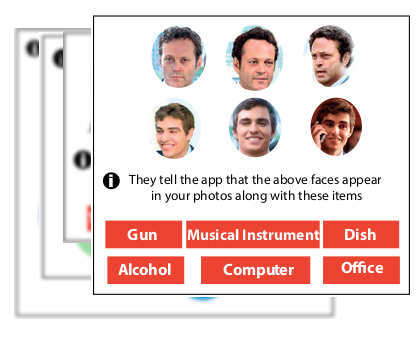
\includegraphics[width=0.8\textwidth]{images/fr4.png}\cite{paper} % , height=0.8\textheight
    \end{center}
}
\frame{
	\frametitle{New permission models: FR}
	\begin{center}
    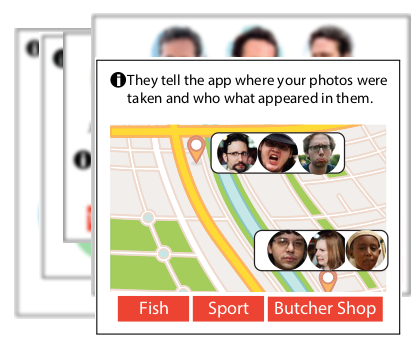
\includegraphics[width=0.8\textwidth]{images/fr5.png}\cite{paper} % , height=0.8\textheight
    \end{center}
}

{
\section*{}
	\begin{frame}
      \begin{center}
        \font\endfont = cmss10 at 10.40mm
        \color{darkBlue}
        \endfont 
        \baselineskip 20.0mm   
        Permission model study
      \end{center}    
\end{frame}
}

\section{Permission model study}
\frame{
	\frametitle{Permission model study}
	210 participants \vspace{5mm} \\
	Four groups: DP (50), IM (54), FR (51), Control Group (55) \vspace{5mm} \\
	Procedure: Person confronted with an app and the wanted permissions $\Rightarrow$ Would you install?
}
\frame{
	\frametitle{Permission model study}
	\begin{center}
    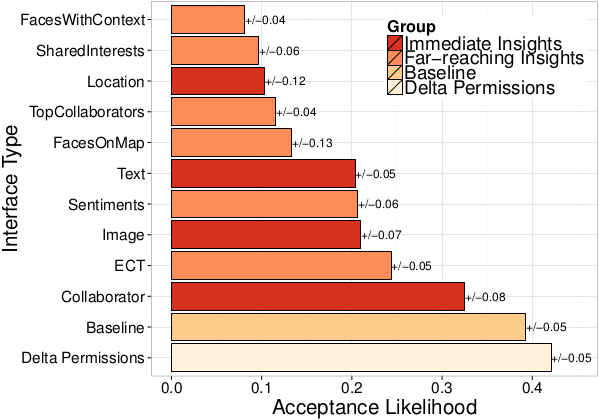
\includegraphics[width=1\textwidth]{images/alResults.png}\cite{paper} % , height=0.8\textheight
    \end{center}
}

{
\section*{}
	\begin{frame}
      \begin{center}
        \font\endfont = cmss10 at 10.40mm
        \color{darkBlue}
        \endfont 
        \baselineskip 20.0mm   
        PrivySeal
      \end{center}    
\end{frame}
}

\section{PrivySeal}
\frame{
	\frametitle{PrivySeal}
	App store developed by the authors \vspace{5mm} \\
	Focus on protection of the user's privacy \vspace{5mm} \\
	Three core feature \vspace{5mm} \\
	1440 registered users (effective 2016) \vspace{5mm} \\
	100 apps (effective 2016)
}

{
\section*{}
	\begin{frame}
      \begin{center}
        \font\endfont = cmss10 at 10.40mm
        \color{darkBlue}
        \endfont 
        \baselineskip 20.0mm   
        Current misbehaviour of developers
      \end{center}    
\end{frame}
}

\section{Current misbehaviour of developers}
\frame{
	\frametitle{Current misbehaviour of developers: How have the permissions changed?}
%	Analysis of previously installed apps from their app store users $\Rightarrow$ 662 apps from three sources \vspace{5mm} \\
Analysis 662 apps from three sources \vspace{5mm} \\
	Google Chrome Web Store: 159 apps \vspace{5mm} \\
	Other Google Web Stores : 66 apps \vspace{5mm} \\
	Outside of Google Web Stores: 437 apps
}
\frame{
	\frametitle{Current misbehaviour of developers: How have the permissions changed?}
	\begin{center}
    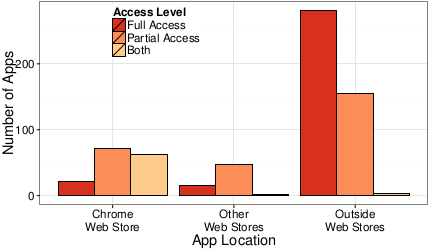
\includegraphics[width=1\textwidth]{images/changeOfAccess.png}\cite{paper} % , height=0.8\textheight
    \end{center}
}
\frame{
	\frametitle{Current misbehaviour of developers: The importance of metadata}
	Analysis of the informations that can be gained by accessing the users metadata \vspace{5mm} \\
	200 registered users with each more than ten text files \vspace{5mm} \\
	''General Topics``: 78 percent matches \vspace{5mm} \\
	''Specific Topics``: 66 percent matches \vspace{5mm} \\
	''Concepts``: 31 percent matches but 69 percent are mostly similar
}

{
\section*{}
	\begin{frame}
      \begin{center}
        \font\endfont = cmss10 at 10.40mm
        \color{darkBlue}
        \endfont 
        \baselineskip 20.0mm   
        Best practices
      \end{center}    
\end{frame}
}

\section{Best practices}
\frame{
	\frametitle{Best practices}
	Use more granulated permissions \vspace{5mm} \\
	Add an overview to cloud platforms \vspace{5mm} \\
	Inform users about insights that could be gained \vspace{5mm} \\
	Add an additional API 
}

{
\section*{}
	\begin{frame}
      \begin{center}
        \font\endfont = cmss10 at 10.40mm
        \color{darkBlue}
        \endfont 
        \baselineskip 20.0mm   
        Influence
      \end{center}    
\end{frame}
}

\section{Influence}
\frame{
	\frametitle{Influence}
}

{
\section*{}
	\begin{frame}
      \begin{center}
        \font\endfont = cmss10 at 10.40mm
        \color{darkBlue}
        \endfont 
        \baselineskip 20.0mm
        Thank you for your attention!
      \end{center}    
\end{frame}
}

\appendix

{
\section*{}
	\begin{frame}
      \begin{center}
        \font\endfont = cmss10 at 10.40mm
        \color{darkBlue}
        \endfont 
        \baselineskip 20.0mm
        References
      \end{center}    
\end{frame}
}

%\addtocounter{framenumber}{-16}
\section{References}
\begin{frame}[allowframebreaks]
\frametitle{References}
\small{
\begin{thebibliography}{99} 
\bibitem{paper}
  Hamza Harkous and Rameez Rahman and Bojan Karlas and Karl Aberer, \emph{The Curious Case of the PDF Converter that Likes Mozart: Dissecting and Mitigating the Privacy Risk of Personal Cloud Apps}, \url{https://petsymposium.org/2016/files/papers/The\_Curious\_Case\_of\_the\_PDF\_Converter\_that\_Likes\_Mozart\_\_Dissecting\_and\_Mitigating\_the\_Privacy\_Risk\_of\_Personal\_Cloud\_Apps.pdf}
\end{thebibliography}
}
\end{frame}

\end{document}